\documentclass{standalone}
\usepackage{tikz}
\usetikzlibrary{patterns, positioning}
\usepackage[sfdefault]{ClearSans} %% option 'sfdefault' activates Clear Sans as the default text font
\usepackage[T1]{fontenc}

\begin{document}
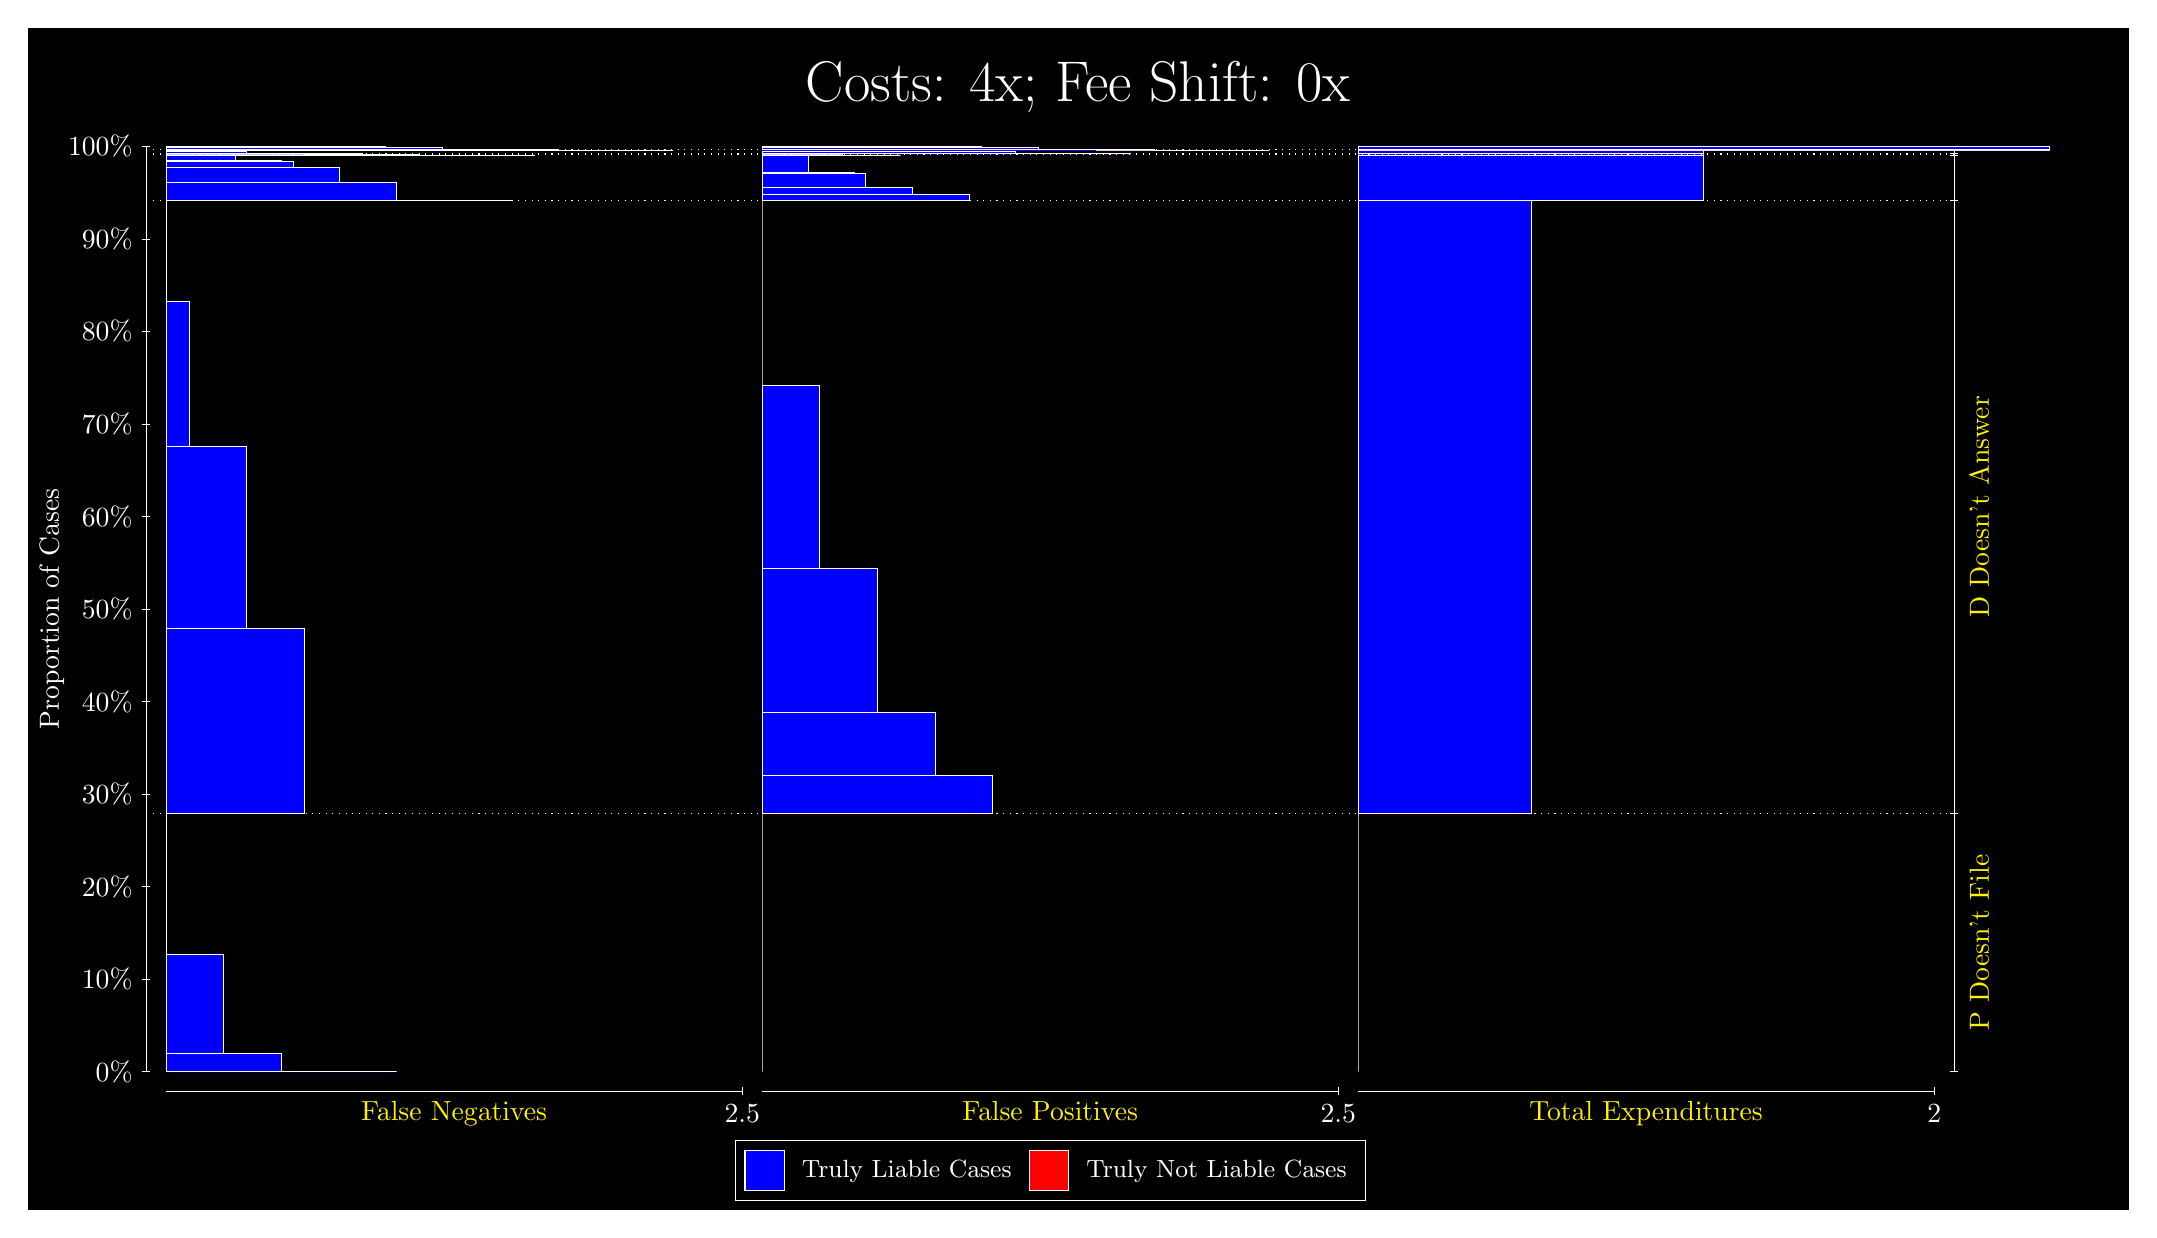
\begin{tikzpicture}
\draw[fill=black] (0,0) rectangle (26.667,15);
\draw[text=white] (0,13.5) rectangle (26.667,15) node[midway] {\huge Costs: 4x; Fee Shift: 0x};
\draw[white, very thin] (1.5,1.75) -- (1.5,13.5);
\node[rotate=90, text=white, anchor=center] at (0.3, 7.625) {Proportion of Cases};
\draw[white, very thin] (1.45,1.75) -- (1.55,1.75);
\node[text=white, anchor=east] at (1.45, 1.75) {0\%};
\draw[white, very thin] (1.45,2.925) -- (1.55,2.925);
\node[text=white, anchor=east] at (1.45, 2.925) {10\%};
\draw[white, very thin] (1.45,4.1) -- (1.55,4.1);
\node[text=white, anchor=east] at (1.45, 4.1) {20\%};
\draw[white, very thin] (1.45,5.275) -- (1.55,5.275);
\node[text=white, anchor=east] at (1.45, 5.275) {30\%};
\draw[white, very thin] (1.45,6.45) -- (1.55,6.45);
\node[text=white, anchor=east] at (1.45, 6.45) {40\%};
\draw[white, very thin] (1.45,7.625) -- (1.55,7.625);
\node[text=white, anchor=east] at (1.45, 7.625) {50\%};
\draw[white, very thin] (1.45,8.8) -- (1.55,8.8);
\node[text=white, anchor=east] at (1.45, 8.8) {60\%};
\draw[white, very thin] (1.45,9.975) -- (1.55,9.975);
\node[text=white, anchor=east] at (1.45, 9.975) {70\%};
\draw[white, very thin] (1.45,11.15) -- (1.55,11.15);
\node[text=white, anchor=east] at (1.45, 11.15) {80\%};
\draw[white, very thin] (1.45,12.325) -- (1.55,12.325);
\node[text=white, anchor=east] at (1.45, 12.325) {90\%};
\draw[white, very thin] (1.45,13.5) -- (1.55,13.5);
\node[text=white, anchor=east] at (1.45, 13.5) {100\%};

\draw[white, very thin] (24.457,1.75) -- (24.457,13.5);
\draw[white, very thin] (24.407,1.75) -- (24.507,1.75);
\node[anchor=west] at (24.407, 1.75) {};
\draw[white, very thin] (24.407,5.0254) -- (24.507,5.0254);
\node[anchor=west] at (24.407, 5.0254) {};
\draw[white, very thin] (24.407,12.817) -- (24.507,12.817);
\node[anchor=west] at (24.407, 12.817) {};
\draw[white, very thin] (24.407,13.391) -- (24.507,13.391);
\node[anchor=west] at (24.407, 13.391) {};
\draw[white, very thin] (24.407,13.408) -- (24.507,13.408);
\node[anchor=west] at (24.407, 13.408) {};
\draw[white, very thin] (24.407,13.456) -- (24.507,13.456);
\node[anchor=west] at (24.407, 13.456) {};
\draw[white, very thin] (24.407,13.5) -- (24.507,13.5);
\node[anchor=west] at (24.407, 13.5) {};

\draw[white, very thin, fill=blue] (1.75,1.75) rectangle (4.6775,1.75);
\draw[white, very thin, fill=blue] (1.75,1.75) rectangle (3.9457,1.7519);
\draw[white, very thin, fill=blue] (1.75,1.7519) rectangle (3.2138,1.9763);
\draw[white, very thin, fill=blue] (1.75,1.9763) rectangle (2.4819,3.2363);
\draw[white, very thin, fill=red] (1.75,3.2363) rectangle (1.75,3.2363);
\draw[white, very thin, fill=blue] (1.75,3.2363) rectangle (1.75,5.0254);
\draw[white, very thin, fill=blue] (1.75,5.0254) rectangle (3.5065,7.3751);
\draw[white, very thin, fill=blue] (1.75,7.3751) rectangle (2.7746,9.6951);
\draw[white, very thin, fill=blue] (1.75,9.6951) rectangle (2.0428,11.528);
\draw[white, very thin, fill=red] (1.75,11.528) rectangle (1.75,11.528);
\draw[white, very thin, fill=blue] (1.75,11.528) rectangle (1.75,12.817);
\draw[white, very thin, fill=blue] (1.75,12.817) rectangle (6.1413,12.817);
\draw[white, very thin, fill=blue] (1.75,12.817) rectangle (5.5558,12.817);
\draw[white, very thin, fill=blue] (1.75,12.817) rectangle (5.4094,12.821);
\draw[white, very thin, fill=blue] (1.75,12.821) rectangle (4.8239,12.821);
\draw[white, very thin, fill=blue] (1.75,12.821) rectangle (4.6775,13.041);
\draw[white, very thin, fill=blue] (1.75,13.041) rectangle (4.092,13.046);
\draw[white, very thin, fill=blue] (1.75,13.046) rectangle (3.9457,13.229);
\draw[white, very thin, fill=blue] (1.75,13.229) rectangle (3.3602,13.315);
\draw[white, very thin, fill=blue] (1.75,13.315) rectangle (3.2138,13.318);
\draw[white, very thin, fill=blue] (1.75,13.318) rectangle (2.6283,13.391);
\draw[white, very thin, fill=red] (1.75,13.391) rectangle (1.75,13.391);
\draw[white, very thin, fill=blue] (1.75,13.391) rectangle (6.4341,13.391);
\draw[white, very thin, fill=blue] (1.75,13.391) rectangle (5.7022,13.391);
\draw[white, very thin, fill=blue] (1.75,13.391) rectangle (4.9703,13.4);
\draw[white, very thin, fill=blue] (1.75,13.4) rectangle (4.2384,13.408);
\draw[white, very thin, fill=blue] (1.75,13.408) rectangle (3.5065,13.408);
\draw[white, very thin, fill=red] (1.75,13.408) rectangle (1.75,13.408);
\draw[white, very thin, fill=blue] (1.75,13.408) rectangle (3.5065,13.408);
\draw[white, very thin, fill=blue] (1.75,13.408) rectangle (2.7746,13.431);
\draw[white, very thin, fill=blue] (1.75,13.431) rectangle (2.0428,13.454);
\draw[white, very thin, fill=red] (1.75,13.454) rectangle (1.75,13.454);
\draw[white, very thin, fill=blue] (1.75,13.454) rectangle (1.75,13.456);
\draw[white, very thin, fill=blue] (1.75,13.456) rectangle (8.1906,13.456);
\draw[white, very thin, fill=blue] (1.75,13.456) rectangle (7.4587,13.456);
\draw[white, very thin, fill=blue] (1.75,13.456) rectangle (6.7268,13.457);
\draw[white, very thin, fill=blue] (1.75,13.457) rectangle (5.9949,13.467);
\draw[white, very thin, fill=blue] (1.75,13.467) rectangle (5.2631,13.489);
\draw[white, very thin, fill=blue] (1.75,13.489) rectangle (4.5312,13.499);
\draw[white, very thin, fill=blue] (1.75,13.499) rectangle (3.7993,13.5);
\draw[white, very thin, fill=blue] (1.75,13.5) rectangle (3.0674,13.5);
\draw[white, very thin, fill=blue] (1.75,13.5) rectangle (2.3355,13.5);
\draw[white, very thin, fill=red] (1.75,13.5) rectangle (1.75,13.5);
\draw[white, very thin, fill=red] (9.3189,1.75) rectangle (9.3189,1.75);
\draw[white, very thin, fill=blue] (9.3189,1.75) rectangle (9.3189,5.0254);
\draw[white, very thin, fill=red] (9.3189,5.0254) rectangle (12.246,5.0254);
\draw[white, very thin, fill=blue] (9.3189,5.0254) rectangle (12.246,5.5102);
\draw[white, very thin, fill=blue] (9.3189,5.5102) rectangle (11.515,6.3143);
\draw[white, very thin, fill=blue] (9.3189,6.3143) rectangle (10.783,8.1474);
\draw[white, very thin, fill=blue] (9.3189,8.1474) rectangle (10.051,10.467);
\draw[white, very thin, fill=blue] (9.3189,10.467) rectangle (9.3189,12.817);
\draw[white, very thin, fill=red] (9.3189,12.817) rectangle (11.954,12.817);
\draw[white, very thin, fill=blue] (9.3189,12.817) rectangle (11.954,12.891);
\draw[white, very thin, fill=red] (9.3189,12.891) rectangle (11.368,12.891);
\draw[white, very thin, fill=blue] (9.3189,12.891) rectangle (11.368,12.893);
\draw[white, very thin, fill=blue] (9.3189,12.893) rectangle (11.222,12.979);
\draw[white, very thin, fill=blue] (9.3189,12.979) rectangle (10.636,13.162);
\draw[white, very thin, fill=blue] (9.3189,13.162) rectangle (10.49,13.167);
\draw[white, very thin, fill=blue] (9.3189,13.167) rectangle (9.9044,13.387);
\draw[white, very thin, fill=blue] (9.3189,13.387) rectangle (9.758,13.387);
\draw[white, very thin, fill=blue] (9.3189,13.387) rectangle (9.3189,13.391);
\draw[white, very thin, fill=red] (9.3189,13.391) rectangle (11.075,13.391);
\draw[white, very thin, fill=blue] (9.3189,13.391) rectangle (11.075,13.391);
\draw[white, very thin, fill=blue] (9.3189,13.391) rectangle (10.344,13.4);
\draw[white, very thin, fill=blue] (9.3189,13.4) rectangle (9.6116,13.408);
\draw[white, very thin, fill=blue] (9.3189,13.408) rectangle (9.3189,13.408);
\draw[white, very thin, fill=red] (9.3189,13.408) rectangle (14.003,13.408);
\draw[white, very thin, fill=blue] (9.3189,13.408) rectangle (14.003,13.408);
\draw[white, very thin, fill=blue] (9.3189,13.408) rectangle (13.271,13.411);
\draw[white, very thin, fill=blue] (9.3189,13.411) rectangle (12.539,13.434);
\draw[white, very thin, fill=blue] (9.3189,13.434) rectangle (11.807,13.456);
\draw[white, very thin, fill=blue] (9.3189,13.456) rectangle (11.075,13.456);
\draw[white, very thin, fill=red] (9.3189,13.456) rectangle (15.759,13.456);
\draw[white, very thin, fill=blue] (9.3189,13.456) rectangle (15.759,13.456);
\draw[white, very thin, fill=blue] (9.3189,13.456) rectangle (15.028,13.456);
\draw[white, very thin, fill=red] (9.3189,13.456) rectangle (15.028,13.456);
\draw[white, very thin, fill=blue] (9.3189,13.456) rectangle (15.028,13.456);
\draw[white, very thin, fill=blue] (9.3189,13.456) rectangle (14.296,13.457);
\draw[white, very thin, fill=red] (9.3189,13.457) rectangle (14.296,13.457);
\draw[white, very thin, fill=blue] (9.3189,13.457) rectangle (14.296,13.457);
\draw[white, very thin, fill=blue] (9.3189,13.457) rectangle (13.564,13.458);
\draw[white, very thin, fill=red] (9.3189,13.458) rectangle (13.564,13.458);
\draw[white, very thin, fill=blue] (9.3189,13.458) rectangle (13.564,13.467);
\draw[white, very thin, fill=blue] (9.3189,13.467) rectangle (12.832,13.467);
\draw[white, very thin, fill=red] (9.3189,13.467) rectangle (12.832,13.467);
\draw[white, very thin, fill=blue] (9.3189,13.467) rectangle (12.832,13.489);
\draw[white, very thin, fill=blue] (9.3189,13.489) rectangle (12.1,13.499);
\draw[white, very thin, fill=blue] (9.3189,13.499) rectangle (11.368,13.5);
\draw[white, very thin, fill=blue] (9.3189,13.5) rectangle (10.636,13.5);
\draw[white, very thin, fill=blue] (9.3189,13.5) rectangle (9.9044,13.5);
\draw[white, very thin, fill=red] (16.888,1.75) rectangle (16.888,1.75);
\draw[white, very thin, fill=blue] (16.888,1.75) rectangle (16.888,5.0254);
\draw[white, very thin, fill=red] (16.888,5.0254) rectangle (19.083,5.0254);
\draw[white, very thin, fill=blue] (16.888,5.0254) rectangle (19.083,12.817);
\draw[white, very thin, fill=red] (16.888,12.817) rectangle (21.279,12.817);
\draw[white, very thin, fill=blue] (16.888,12.817) rectangle (21.279,13.391);
\draw[white, very thin, fill=red] (16.888,13.391) rectangle (21.279,13.391);
\draw[white, very thin, fill=blue] (16.888,13.391) rectangle (21.279,13.408);
\draw[white, very thin, fill=red] (16.888,13.408) rectangle (21.279,13.408);
\draw[white, very thin, fill=blue] (16.888,13.408) rectangle (21.279,13.456);
\draw[white, very thin, fill=red] (16.888,13.456) rectangle (25.67,13.456);
\draw[white, very thin, fill=blue] (16.888,13.456) rectangle (25.67,13.457);
\draw[white, very thin, fill=red] (16.888,13.457) rectangle (25.67,13.457);
\draw[white, very thin, fill=blue] (16.888,13.457) rectangle (25.67,13.5);
\draw[white, dotted] (1.5,5.0254) -- (24.457,5.0254);
\draw[white, dotted] (1.5,12.817) -- (24.457,12.817);
\draw[white, dotted] (1.5,13.391) -- (24.457,13.391);
\draw[white, dotted] (1.5,13.408) -- (24.457,13.408);
\draw[white, dotted] (1.5,13.456) -- (24.457,13.456);
\draw[white, very thin] (1.75,1.5) -- (9.0689,1.5);
\node[text=yellow, anchor=north] at (5.4094, 1.5) {False Negatives};
\draw[white, very thin] (9.0689,1.45) -- (9.0689,1.55);
\node[text=white, anchor=north] at (9.0689, 1.45) {2.5};

\draw[white, very thin] (9.3189,1.5) -- (16.638,1.5);
\node[text=yellow, anchor=north] at (12.978, 1.5) {False Positives};
\draw[white, very thin] (16.638,1.45) -- (16.638,1.55);
\node[text=white, anchor=north] at (16.638, 1.45) {2.5};

\draw[white, very thin] (16.888,1.5) -- (24.207,1.5);
\node[text=yellow, anchor=north] at (20.547, 1.5) {Total Expenditures};
\draw[white, very thin] (24.207,1.45) -- (24.207,1.55);
\node[text=white, anchor=north] at (24.207, 1.45) {2};

\node[text=yellow, centered, rotate=90] at (24.777, 3.3877) {P Doesn't File};
\node[text=yellow, centered, rotate=90] at (24.777, 8.9213) {D Doesn't Answer};





\draw (12.978300999999998,1.5) node[draw=none] (baseCoordinate) {};
\begin{scope}[align=center]
        \matrix[scale=0.5, draw=white, below=0.5cm of baseCoordinate, nodes={draw}, column sep=0.1cm]{
            \node[rectangle, draw, minimum width=0.5cm, minimum height=0.5cm, fill=blue] {}; &
            \node[draw=none, font=\small, text=white] (B) {Truly Liable Cases}; &
            \node[rectangle, draw, minimum width=0.5cm, minimum height=0.5cm, fill=red] {}; &
            \node[draw=none, font=\small, text=white] (B) {Truly Not Liable Cases}; \\
            };
\end{scope}

\end{tikzpicture}
\end{document}